
\documentclass{beamer}
\usepackage[spanish]{babel}
\usepackage{amsthm}
\usepackage{bbding}
\usepackage[utf8]{inputenc}

\mode<presentation> {
\usetheme{Madrid}
}
\usepackage{color}
\usepackage{graphicx} % Allows including images
\usepackage{booktabs} % Allows the use of \toprule, \midrule and \bottomrule in tables
\setbeamertemplate{blocks}[rounded][shadow=true]
%----------------------------------------------------------------------------------------
%	TITLE PAGE
%----------------------------------------------------------------------------------------

\title[Presentación del TP2]{Semántica Web} % The short title appears at the bottom of every slide, the full title is only on the title page

\author{Bases de Datos} % Your name
\institute[] % Your institution as it will appear on the bottom of every slide, may be shorthand to save space
{
Federico Allocati, Sabrina Izcovich, Santiago Pernigotti, Germán Romano\\ % Your institution for the title page
\medskip
%\textit{john@smith.com} % Your email address
}
\date{Miércoles 8 de julio de 2015} % Date, can be changed to a custom date

\begin{document}

\begin{frame}
\titlepage % Print the title page as the first slide
\end{frame}

\begin{frame}
\frametitle{Contenidos} % Table of contents slide, comment this block out to remove it
\tableofcontents % Throughout your presentation, if you choose to use \section{} and \subsection{} commands, these will automatically be printed on this slide as an overview of your presentation
\end{frame}

%----------------------------------------------------------------------------------------
%	PRESENTATION SLIDES
%----------------------------------------------------------------------------------------

%------------------------------------------------
\section{Introducción} 
%------------------------------------------------
\begin{frame}
\frametitle{Material Analizado}
\begin{itemize}
\item \textbf{Optimizing Reformulated RDF Queries}, Damián A. Bursztyn, 2013

\end{itemize}
\end{frame}

%------------------------------------------------
\section{Contextualizando...} 
%------------------------------------------------
\subsection{Web Semántica}
\begin{frame}
\frametitle{¿Qué es la Web Semántica?} 
\begin{block}{Web Semántica}
\begin{itemize}
\item<1-> Web Extendida enfocada en el significado de las búsquedas.
\item<2-> Se procesa la información en términos de su semántica a través de operaciones bien definidas.
\item<3-> El software es capaz de procesar el contenido, razonar con este, combinarlo y realizar deducciones lógicas para resolver problemas cotidianos automáticamente.
\item<4-> Utiliza una infraestructura común mediante la cual es posible compartir, procesar y transferir información de forma sencilla.
\item<5-> Otorga una solución a problemas habituales en la búsqueda de información ocasionados por la sobrecarga de información y heterogeneidad de fuentes de información.
\end{itemize}
\end{block}
\end{frame}
%------------------------------------------------
\begin{frame}
\frametitle{Ejemplo} 
\begin{figure}[H] %[h] Aqui [b] para button [t] para top
\begin{center}
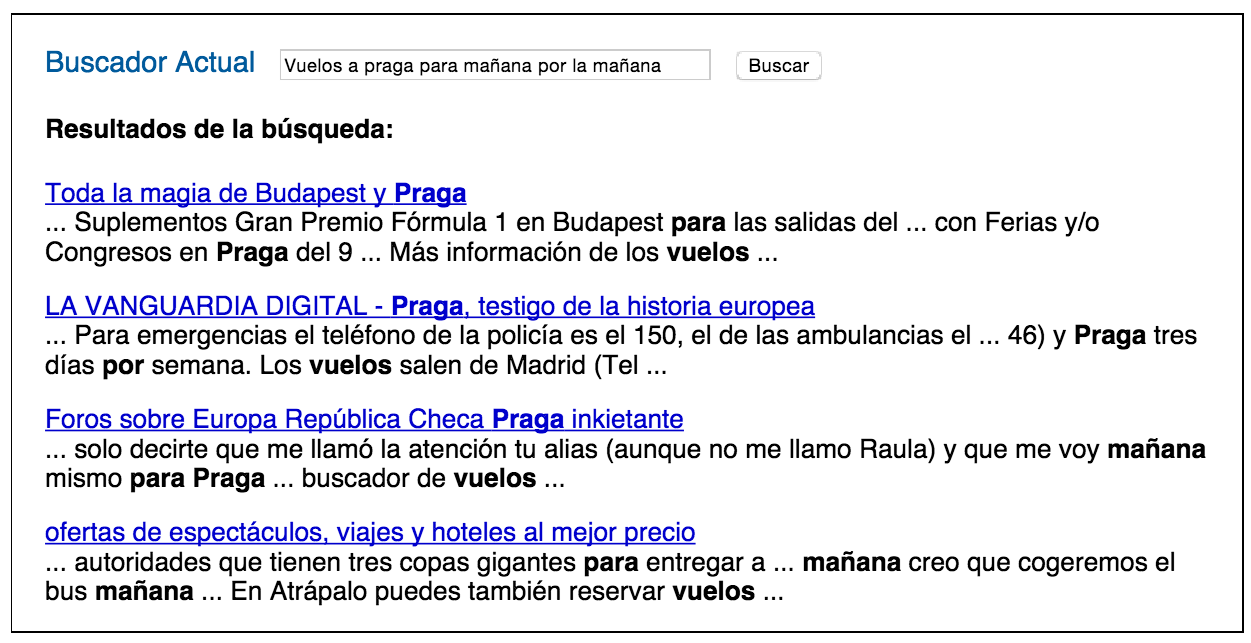
\includegraphics[width=340pt]{resultadoNormal.png}
\caption{Resultados obtenidos con un buscador normal.}
\end{center}
\end{figure}
\end{frame}
%------------------------------------------------
\begin{frame}
\frametitle{Ejemplo} 
\begin{figure}[H] %[h] Aqui [b] para button [t] para top
\begin{center}
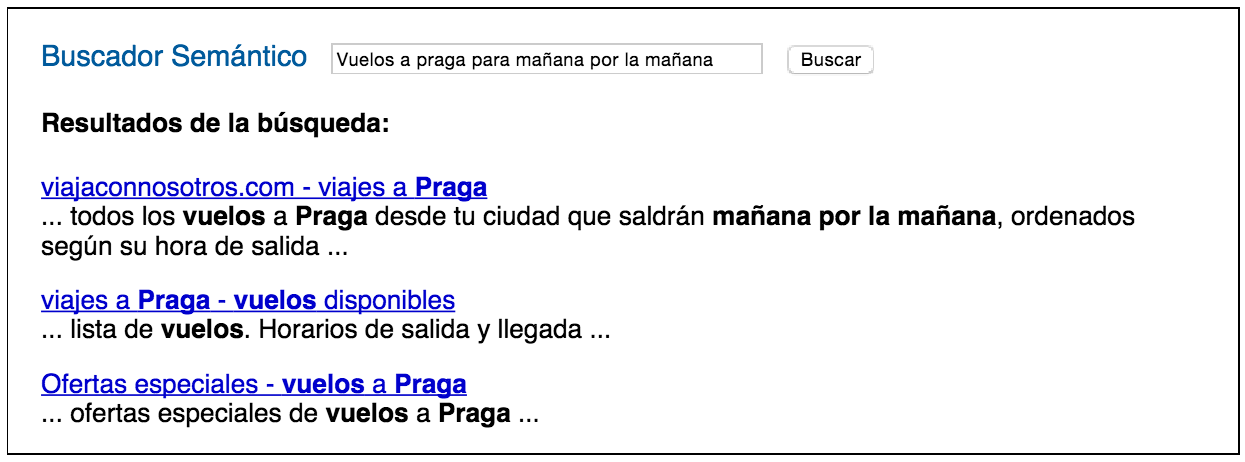
\includegraphics[width=340pt]{resultadoSemantico.png}
\caption{Resultados obtenidos con un buscador semántico.}
\end{center}
\end{figure}
\end{frame}
%------------------------------------------------
\subsection{RDF}
\begin{frame}[fragile] % Need to use the fragile option when verbatim is used in the slide
\frametitle{¿Qué es RDF?}
\begin{block}{Resource Description Framework}
\begin{itemize}
\item<1-> Es un grafo dirigido etiquetado para representar información en la Web en donde los ejes representan la relación entre dos fuentes (los nodos).
\item<2-> En particular, es el formato para modelar el intercambio de datos en la web semántica. 
\item<3-> Tiene características que facilitan la fusión de datos a pesar de que sus esquemas de organización difieran.
\item<4-> Extiende la unión de estructuras en la Web nombrando las relaciones entre cosas.
\item<5-> Su utilización permite estructurar los datos a ser fusionados, expuestos y compartidos a través de diferentes aplicaciones.
\end{itemize}
\end{block}
\end{frame}

%------------------------------------------------
\begin{frame}[fragile]
\frametitle{Ejemplo}
\textit{``Javier Perez es el autor del documento cuya URL es http://www.dc.uba.ar/examen.pdf. Su mail es jperez@dc.uba.ar y su teléfono +54(11)4563-4567.''}
\begin{verbatim}
<?namespace href="http://dc.uba.ar/info-bibliografia" as="bib"?> 
<RDF:serialization> 
  <RDF:assertions href="http://dc.uba.ar/examen.pdf"> 
    <bib:autor> 
      <RDF:resource> 
        <bib:nombre>Javier Perez</bib:nombre> 
        <bib:mail>jperez@dc.uba.ar</bib:mail> 
        <bib:telefono>+54(11)4563-4567</bib:telefono> 
      </RDF:resource> 
    </bib:autor> 
  </RDF:assertions> 
</RDF:serialization>

\end{verbatim}
\end{frame}

%------------------------------------------------
\begin{frame}[fragile]
\frametitle{Ejemplo} 
\begin{center}
\begin{figure}[H] %[h] Aqui [b] para button [t] para top
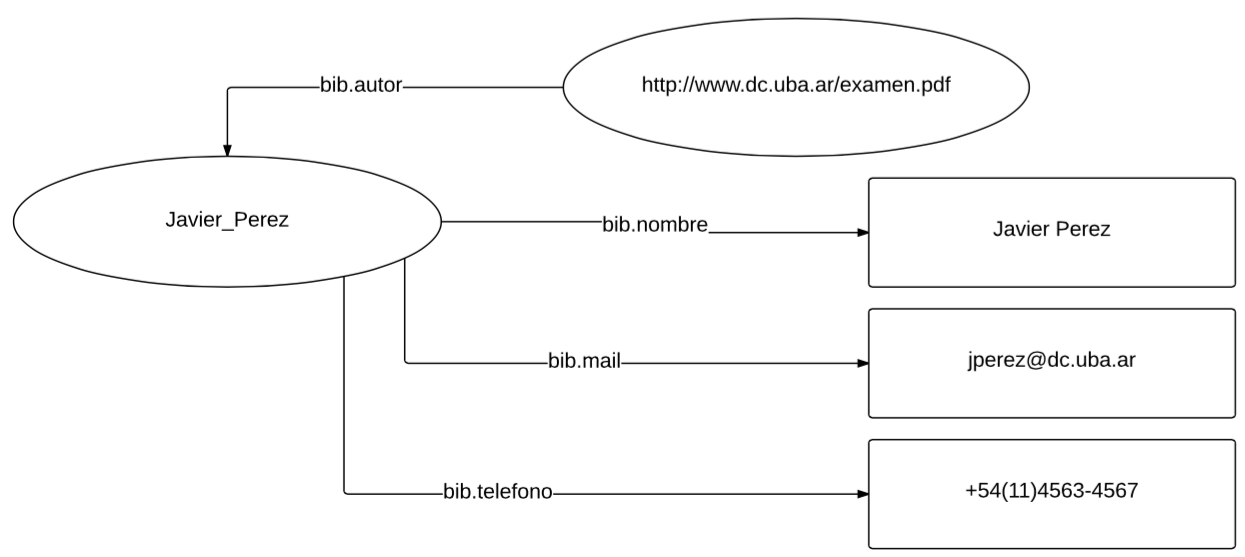
\includegraphics[width=300pt]{rdfModel.png}
\caption{Modelo RDF.}
\end{figure}
Los nodos son las elipses, los ejes la relación y los rectángulos son strings.
\end{center}
\end{frame}
%------------------------------------------------

\begin{frame}
\frametitle{Queries BGP y SPARQL}
\begin{exampleblock}{Basic Graph Pattern}


\end{exampleblock}

\begin{exampleblock}{SPARQL}
Es el estándar W3C para consultas RDF.

\end{exampleblock}
\end{frame}
%------------------------------------------------
\begin{frame}
\frametitle{RDF y RDBMs}
%------------------------------------------------
\begin{block}{RDF y RDBMS}
\begin{itemize}
\item{Es posible transformar una consulta BGP en otra capaz de ser evaluada por RDBMS.}
\item{Se almacenan los triples dentro de tablas y se reformula la consulta BGP por una equivalente.}
\item{$q(x) : s_{1} p_{1} o_{1}, ..., s_{n} p_{n} o_{n}$ es equivalente a $q(x): \wedge ^n _{i = 1} Triples(s_{i}, p_{i}, o_{i})$}
\item{Para resolver la consulta se empelean dos técnicas de manejo de vinculos RDF: Saturación o Reformulación.}
\end{itemize}
\end{block}
\end{frame}
%------------------------------------------------

\begin{frame}
\frametitle{RDF y RDBMs}

\begin{figure}[h]
\begin{center}
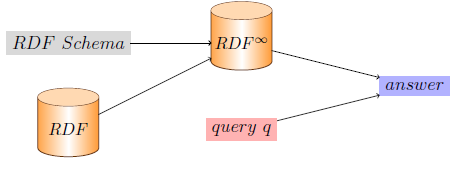
\includegraphics[width=200pt]{saturacion}
\caption{Visión general del proceso de respuesta de una consulta basada en saturación.}
\end{center}
\end{figure}

\begin{figure}[H]
\begin{center}
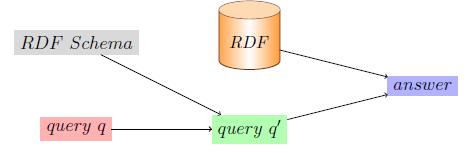
\includegraphics[width=200pt]{reformulacion}
\caption{Visión general del proceso de respuesta de una consulta basada en reformulación.}
\end{center}
\end{figure}
\end{frame}

%------------------------------------------------
\begin{frame}
\frametitle{Reformulación de queries}

\end{frame}
%------------------------------------------------
\begin{frame}
\frametitle{Temas especiales en Semántica Web}

\end{frame}
%------------------------------------------------

\begin{frame}
\Huge{\centerline{¿Preguntas?}}
\end{frame}

%----------------------------------------------------------------------------------------

\end{document} 
